%\nonstopmode
\documentclass[aspectratio=169]{beamer}
\usepackage[utf8]{inputenc}
% \usepackage[frenchb]{babel}
\usepackage{amsmath}
\usepackage{mathtools}
\usepackage{breqn}
\usepackage{multirow}
\usetheme{Luebeck}
\usepackage{graphicx}
%\useoutertheme[footline=authortitle,subsection=false]{miniframes}

\beamertemplatenavigationsymbolsempty
\setbeamertemplate{footline}
{%
  \leavevmode%
  \hbox{\begin{beamercolorbox}[wd=.15\paperwidth,ht=2.5ex,dp=1.125ex,leftskip=.3cm,rightskip=.3cm plus1fill]{author in head/foot}%
    \usebeamerfont{author in head/foot} \insertframenumber{} / \inserttotalframenumber
  \end{beamercolorbox}%
  \begin{beamercolorbox}[wd=.2\paperwidth,ht=2.5ex,dp=1.125ex,leftskip=.3cm plus1fill,rightskip=.3cm]{author in head/foot}%
    \usebeamerfont{author in head/foot}\insertshortauthor
  \end{beamercolorbox}%
  \begin{beamercolorbox}[wd=.65\paperwidth,ht=2.5ex,dp=1.125ex,leftskip=.3cm,rightskip=.3cm plus1fil]{title in head/foot}%
    \usebeamerfont{title in head/foot}\insertshorttitle~--~\insertshortdate
  \end{beamercolorbox}}%
  \vskip0pt%
}

\usepackage{tabu}
\usepackage{multicol}
\usepackage{vwcol}
\usepackage{stmaryrd}
\usepackage{graphicx}

\usepackage[normalem]{ulem}

\title[Garage : jouer dans la cour des grands quand on est un hébergeur associatif]{Garage : jouer dans la cour des grands \\quand on est un hébergeur associatif}
\subtitle{(ou pourquoi on a décidé de réinventer la roue)}
\author[Q. Dufour \& A. Auvolat]{Quentin Dufour \& Alex Auvolat}
\date[02/12/2020]{Mercredi 2 décembre 2020}

\begin{document}

\begin{frame}
	\titlepage
\end{frame}

\begin{frame}
	\frametitle{La question qui tue}
	
	\begin{center}
		\includegraphics[scale=3]{img/sync.png} \\
		\Huge Pourquoi vous n'hébergez pas vos fichiers chez vous ? \\
	\end{center}

\end{frame}

\begin{frame}[t]
	\frametitle{La cour des grands}

	\begin{columns}[t]
	\begin{column}{0.5\textwidth}
		{\huge Le modèle du cloud...}
	 
	\begin{center}
		\includegraphics[scale=0.08]{img/cloud.png}
	\end{center}
	
		+ \underline{intégrité} : plus de perte de données
	
		+ \underline{disponibilité} : tout le temps accessible
		
		+ \underline{service} : rien à gérer
	
		\vspace{0.15cm}
		\textbf{changement des comportements}
	\end{column}
	\pause
	\begin{column}{0.5\textwidth}
		{\huge ...et son prix}
	 
	\begin{center}
		\includegraphics[scale=0.07]{img/dc.jpg}
	\end{center}
	
		- matériel couteux et polluant
	
		- logiciels secrets
	
		- gestion opaque
	
		\vspace{0.2cm}
		\textbf{prisonnier de l'écosystème}
	\end{column}
	\end{columns}
\end{frame}

\begin{frame}[t]
	\frametitle{Garage l'imposteur}

	\begin{columns}[t]
	\begin{column}{0.5\textwidth}
		{\huge Ressemble à du cloud...}
	 
	\begin{center}
		\includegraphics[scale=0.5]{img/shh.jpg}
	\end{center}
	
	+ \underline{compatible} avec les apps existantes
	
	+ \underline{fonctionne} avec le mobile
	
	+ \underline{s'adapte} aux habitudes prises
	
	
	\end{column}
	
	\pause
	\begin{column}{0.5\textwidth}
		{\huge ...fait du P2P}
	
	\begin{center}
		\includegraphics[scale=1]{img/death.jpg}
	\end{center}
	
	\vspace{0.4cm}
	
	+ \underline{contrôle} de l'infrastructure
	
	+ \underline{transparent} code libre 
	
	+ \underline{sobre} fonctionne avec de vieilles machines à la maison
	\end{column}
	\end{columns}

\end{frame}


\graphicspath{{img/}}

\begin{frame}
	\frametitle{Mais donc, c'est quoi Garage ?}

	\begin{columns}[t]
	\begin{column}{0.5\textwidth}
		\centering
		\textbf{Un système de stockage distribué}
		\vspace{1em}

			
\includegraphics[width=.7\columnwidth]{img/garage_distributed.pdf}
	\end{column}
	\pause

	\begin{column}{0.5\textwidth}
		\centering
		\textbf{qui implémente l'API S3}
		\vspace{2em}

		\includegraphics[width=.7\columnwidth]{img/Amazon-S3.jpg}
	\end{column}
	\end{columns}
\end{frame}

\begin{frame}
	\frametitle{Consistent Hashing (DynamoDB)}
	\textbf{Comment répartir les fichiers sur les différentes machines ?}
	\vspace{1em}

	\centering

	\only<1>{\includegraphics[width=.55\columnwidth]{img/consistent_hashing_1.pdf}}%
	\only<2>{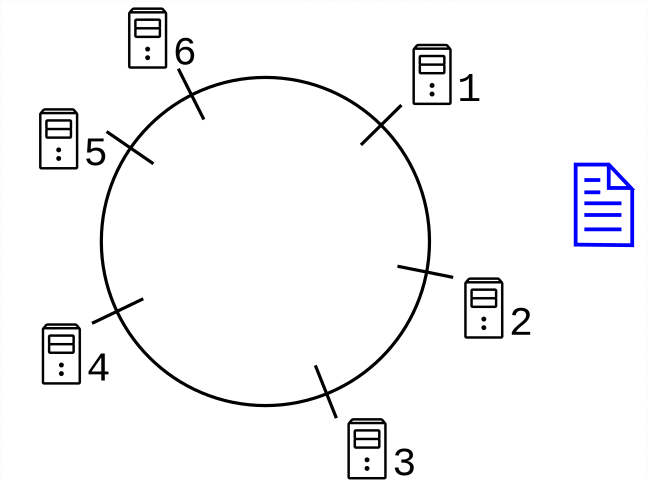
\includegraphics[width=.55\columnwidth]{img/consistent_hashing_2.pdf}}%
	\only<3>{\includegraphics[width=.55\columnwidth]{img/consistent_hashing_3.pdf}}%
	\only<4>{\includegraphics[width=.55\columnwidth]{img/consistent_hashing_4.pdf}}%
\end{frame}

\begin{frame}
	\frametitle{Garage Internals : 3 niveaux de consistent hashing}
	\centering
	\includegraphics[width=.85\columnwidth]{img/garage_tables.pdf}
\end{frame}

\begin{frame}
	\frametitle{Modèles de cohérence}
	Garage utilise un modèle de cohérence relativement faible :
	\vspace{1em}

	\begin{itemize}
		\item Objets répliqués 3 fois, quorum de 2 pour les lectures et les écritures\\
			$\to$ cohérence \textbf{``read your writes''}
			\vspace{1em}
		\item<2-> Types de donnée CRDT + mécanisme d'anti-entropie\\
			$\to$ cohérence \textbf{à terme} (eventual consistency)
			\vspace{1em}
		\item<3-> Cela s'applique pour chaque fichier individuellement :\\
			pas de linéarisabilté ou de cohérence causale entre les opérations\\
			sur des fichiers différents
			\vspace{1em}
		\item<4-> \textbf{Avantage :} convient bien à un déploiement géodistribué (multi-datacenter)
	\end{itemize}
\end{frame}

\begin{frame}
	\frametitle{Rust : retour d'expérience}

	\begin{columns}
	\begin{column}{0.55\textwidth}
		Garage est entièrement écrit en Rust !
		\vspace{2em}

		\textbf{Points forts :}
		\vspace{.5em}
		\begin{itemize}
			\item Langage compilé, très rapide
				\vspace{.5em}
			\item Typage fort, beaucoup de sécurités
				\vspace{.5em}
			\item Le meilleur de plusieurs paradigmes:
				fonctionnel, orienté objet, impératif
				\vspace{.5em}
			\item Un écosytème de librairies très complet:
				serialisation, async/await, http, ...
		\end{itemize}
	\end{column}
	
	\begin{column}{0.45\textwidth}
		\begin{centering}
			\hspace{2em}\includegraphics[width=0.55\columnwidth]{img/rustacean-flat-happy.png}
		\end{centering}

		\vspace{2em}
		\textbf{Points faibles :}
		\vspace{.5em}
		\begin{itemize}
			\item Les temps de compilation...
				\vspace{.5em}
			\item Compliqué à apprendre
		\end{itemize}
		\vspace{2em}
	\end{column}
	\end{columns}

\end{frame}

\end{document}

%% vim: set ts=4 sw=4 tw=0 noet spelllang=fr :
